\documentclass{sig-alt-release-2013}
\usepackage[utf8]{inputenc}
\usepackage{listings}
\usepackage{url}

\DeclareMathOperator{\se}{se}

\conferenceinfo{EVIA}{2014, Tokyo, Japan}
\global\boilerplate{}
\global\copyrightetc{This work was produced by an employee of the U.S. Government during the course of his official duties and is placed in the public domain}
%\global\copyrightetc{This is a blinded conference submission.  Copyright is held by the author}

\title{Computing Confidence Intervals for Common IR Measures}
\author{
  \alignauthor
  Ian Soboroff\\
  \affaddr{National Institute of Standards and Technology}\\
  \affaddr{100 Bureau Drive, Gaithersburg, MD, 20899-8940 USA}\\
  \affaddr{ian.soboroff@nist.gov}\\
}

\begin{document}

% \conferenceinfo{SIGIR'13,} {July 28--August 1, 2013, Dublin, Ireland.} 
% \CopyrightYear{2013} 
% \crdata{978-1-4503-2034-4/13/07} 
% \clubpenalty=10000 
% \widowpenalty = 10000

\maketitle

\begin{abstract}
Confidence intervals quantify the uncertainty in an average and offer a robust alternative to hypothesis testing.  We measure the performance of standard and bootstrapped confidence intervals on a number of common IR measures using several TREC and NTCIR collections.  The performance of an interval is its empirical coverage of the estimated statistic.  We find that both standard and bootstrapped intervals give excellent coverage for all measures except in situations of abysmal retrieval performance.  We recommend using standard confidence intervals when statistical software is handy, and bootstrap percentile intervals as equivalent when no statistical libraries are available.
\end{abstract}

\section{Introduction}

Conventional practice in information retrieval recommends testing the statistical significance of results~\cite{Hull93}. Hull recommended use of diagnostic plots to support the distributional assumptions of parametric tests and noted that Student's t test is quite robust to violations of normality.

However, null-hypothesis significance testing has a number of known problems. Statistical significance does not indicate a large or user-visible effect, but rather that the result is very likely to not be null due to sampling error.  The null hypothesis is a strawman, and a successful test against it offers no inferential support for other comparisons.  Significance is not hard to achieve in IR experiments by simply increasing the topic set size, and topic sets in common test collections are large enough to exhibit significant test results for very small differences in a measure~\cite{Cumming12}.

An alternative to significance testing is computing confidence intervals.  A confidence interval for a statistic (like the mean of average precision scores across all topics in a test collection) indicates the region within which we would plausibly expect that statistic to arise in a given proportion of repeated experiments using data from the same population.  Confidence intervals can be compared for overlap to yield a result similar to a statistical test~\cite{Cumming05}. Many disciplines use confidence intervals rather than statistical tests, and confidence intervals were recently suggested for use in information retrieval settings by Sakai~\cite{Sakai14-forum}.

In this paper, we explore several existing methods for computing confidence intervals on common measures in a number of test collection environments.  We then measure the effectiveness of each interval method by its empirical coverage probability, simulating the long-run accuracy of the interval.  Based on these results, we make recommendations for reporting IR measures in future experiments.

\section{Confidence intervals}

A {\em confidence interval} (CI) indicates the range in which we would reasonably expect a statistic such as mean AP score to occur in the long run in similar experiments.  We select a {\em confidence level} such as $95\%$ and estimate where the mean would fall in 95\% of hypothetically repeated experiments from the same population of topics and documents.

If the population arises from a well-known distribution, then the confidence interval around the mean of that population can be derived directly from the definition of the population distribution.  For the mean of values in a standard normal distribution, a 95\% confidence interval around that mean is defined as:
\[ (\theta - z^{(.975)} \cdot \sigma, \theta - z^{(.025)} \cdot \sigma) \]
where $z^{(\alpha)}$ is the percentile of the standard normal distribution with mean $\theta$ and standard deviation $\sigma$.

Since we don't know the mean and variance of the normal distribution giving rise to our retrieval evaluation scores, we can approximate it using Student's $t$ distribution with $n-1$ degrees of freedom, $n$ being the number of topics:
\[ (\hat{\theta} - t^{(.975)}_{n-1} \cdot \hat{\se}, \hat{\theta} - t^{(.025)}_{n-1} \cdot \hat{\se}) \]
where $\hat{\theta}$ is the sample mean of scores from the topics we observe, and $\hat{\se}$ is the standard error.

As an example, the run {\em weaver1} in the TREC 8 adhoc collection has a  mean average precision of 0.2175 with a standard error of 0.0343.  The 95\% standard confidence interval using the $t$ approximation is $[0.1491, 0.2859]$.

Two confidence intervals can be compared visually, and this comparison can be used like a $t$-test.  If the intervals are for independent means (as they are in the kind of IR experiments we describe here) and they just touch at the endpoints, this is roughly equivalent to a significant test result against the null hypothesis of no difference with $p \approx 0.01$.  A gap indicates $p < 0.01$, and moderate overlap of about half of one side of the interval indicates $p \approx 0.05$~\cite{Cumming12}.  Nevertheless, it should be stressed that computing two confidence intervals is {\em not} the same as performing a t-test; the interval defines the precision of the estimate with respect to the population, providing a basis for inference, and since comparing intervals is an analysis method rather than a test, corrections for multiple comparisons may not be necessary~\cite{Saville90}.

\section{Coverage}

When we refer to a 95\% CI, the ``95\%'' value is the {\em nominal} confidence.  However, we may certainly ask how well that interval actually estimates the behavior of the statistic.  We can do this using a resampling or {\em bootstrap} experiment~\cite{Schall12}.  Bootstrapping involves taking random samples from the available observations in order to estimate properties of the distribution from which those observations arose~\cite{Efron93}.

Given our observations (AP scores) and their known mean, we can draw samples from those observations, compute a confidence interval from the sample and check if the known mean falls within the sample's confidence interval.  If we do this repeatedly and count the proportion of times the sample interval contains the original sample mean, we calculate the {\em empirical coverage} of the interval.

For the {\em weaver1} run, we have fifty average precision scores with a mean of 0.2175.  Our implementation of the coverage computation draws 1000 samples from this run, where each sample is fifty AP scores selected from {\em weaver1} with replacement.  From each sample, we compute its 95\% confidence interval.  The empirical coverage is the fraction  of sample confidence intervals that contain the original MAP score.  This coverage score varies slightly due to sampling; in our experiments, the empirical coverage for the standard interval is 0.919, which is smaller than the nominal coverage 0.95.

\section{Bootstrap intervals}

The bootstrap method can be used to estimate the confidence interval itself.  This technique is especially useful when the statistic of interest has no analytical expression of the confidence interval.  When it does (as in the case of the mean) can serve as a check that distributional assumptions are reasonable.  We investigate three bootstrap confidence interval methods: bootstrap percentile, bootstrap-$t$, and bias-corrected and accelerated (BCa) intervals~\cite{Efron93}.

The simplest bootstrap method for confidence intervals is the {\em percentile} method.  Given the original per-topic scores $x$ with sample mean $\hat{\theta}$, we generate a bootstrap data set $x^\star$ by resampling from $x$ with replacement, and compute the mean $\hat{\theta}^\star$ of each bootstrap sample.  Then, sort the means.  Then, the $1 - 2\alpha$ {\em percentile interval} is exactly the $\alpha$ and $1-\alpha$ percentiles of the bootstrap distribution.  If $\alpha = 0.05$ and we take 5000 bootstrap samples, the lower endpoint of the interval is the 250th ordered value of the bootstrap means, and the upper endpoint is the 5,750th value.  An advantage of this method is that it requires no statistical tables or advanced mathematical support for computing distribution functions.

The second method follows from the definition above of textbook studentized intervals.  The motivation behind Student's $t$ distribution is that means of samples from a standard normal distribution are normally distributed, but only in the limit as the sample size approaches the population size.  For smaller samples and when the variance of the population is unknown, Student's $t$ gives a better approximation.  We can studentize the bootstrap in the same way.  For each bootstrap sample $x^\star_b$ from the original per-topic scores $x$, we compute both the mean $\hat{\theta}^\star_b$ and the standard error $\hat{\se}^\star_b$ of the sample.  We then compute a $Z$-score for each as
$Z^\star(b) = \frac{\hat{\theta}^\star(b) - \hat{\theta}}{\hat{\se}^\star(b)}$.
We then compute or look up the critical values from the $t$ distribution with $n - 1$ degrees of freedom, $\hat{t}^{(1-\alpha)}$ and $\hat{t}^\alpha$, and apply them to the original sample mean and standard error to get the bootstrap-$t$ interval,
\[ (\hat{\theta} - \hat{t}^{(1-\alpha)} \cdot \hat{\se}, \hat{\theta} - \hat{t}^{(\alpha)} \cdot \hat{\se}) \]

The third method we use in this paper is the BCa method, which stands for {\em bias-corrected and accelerated} intervals.  BCa intervals adjust the percentile method intervals with two terms,
\begin{align*}
BCa & : (\hat{\theta}^{\star(\alpha_1)}, \hat{\theta}^{\star(\alpha_2)}) \\
\alpha_1 & = \Phi(\hat{z}_0 + \frac{\hat{z}_0 + z^\alpha}{1 - \hat{a}(\hat{z}_0 + z^\alpha)}) \\
\alpha_2 & = \Phi(\hat{z}_0 + \frac{\hat{z}_0 + z^{(1-\alpha)}}{1 - \hat{a}(\hat{z}_0 + z^{(1-\alpha)})})
\end{align*}
$\Phi$ is the standard normal cumulative distribution function, and $z^\alpha$ is a percentile of the standard normal distribution.  

$\hat{z}_0$ is called the bias-correction term, and $\hat{a}$ is the acceleration.  The bias-correction is computed from the proportion of bootstrap replicate means that are less than the original sample mean $\hat{\theta}$.  The acceleration $\hat{a}$ is more complicated and is computed using another resampling method to estimate the rate of change of the standard error of the sample mean.

\begin{figure}[t!]
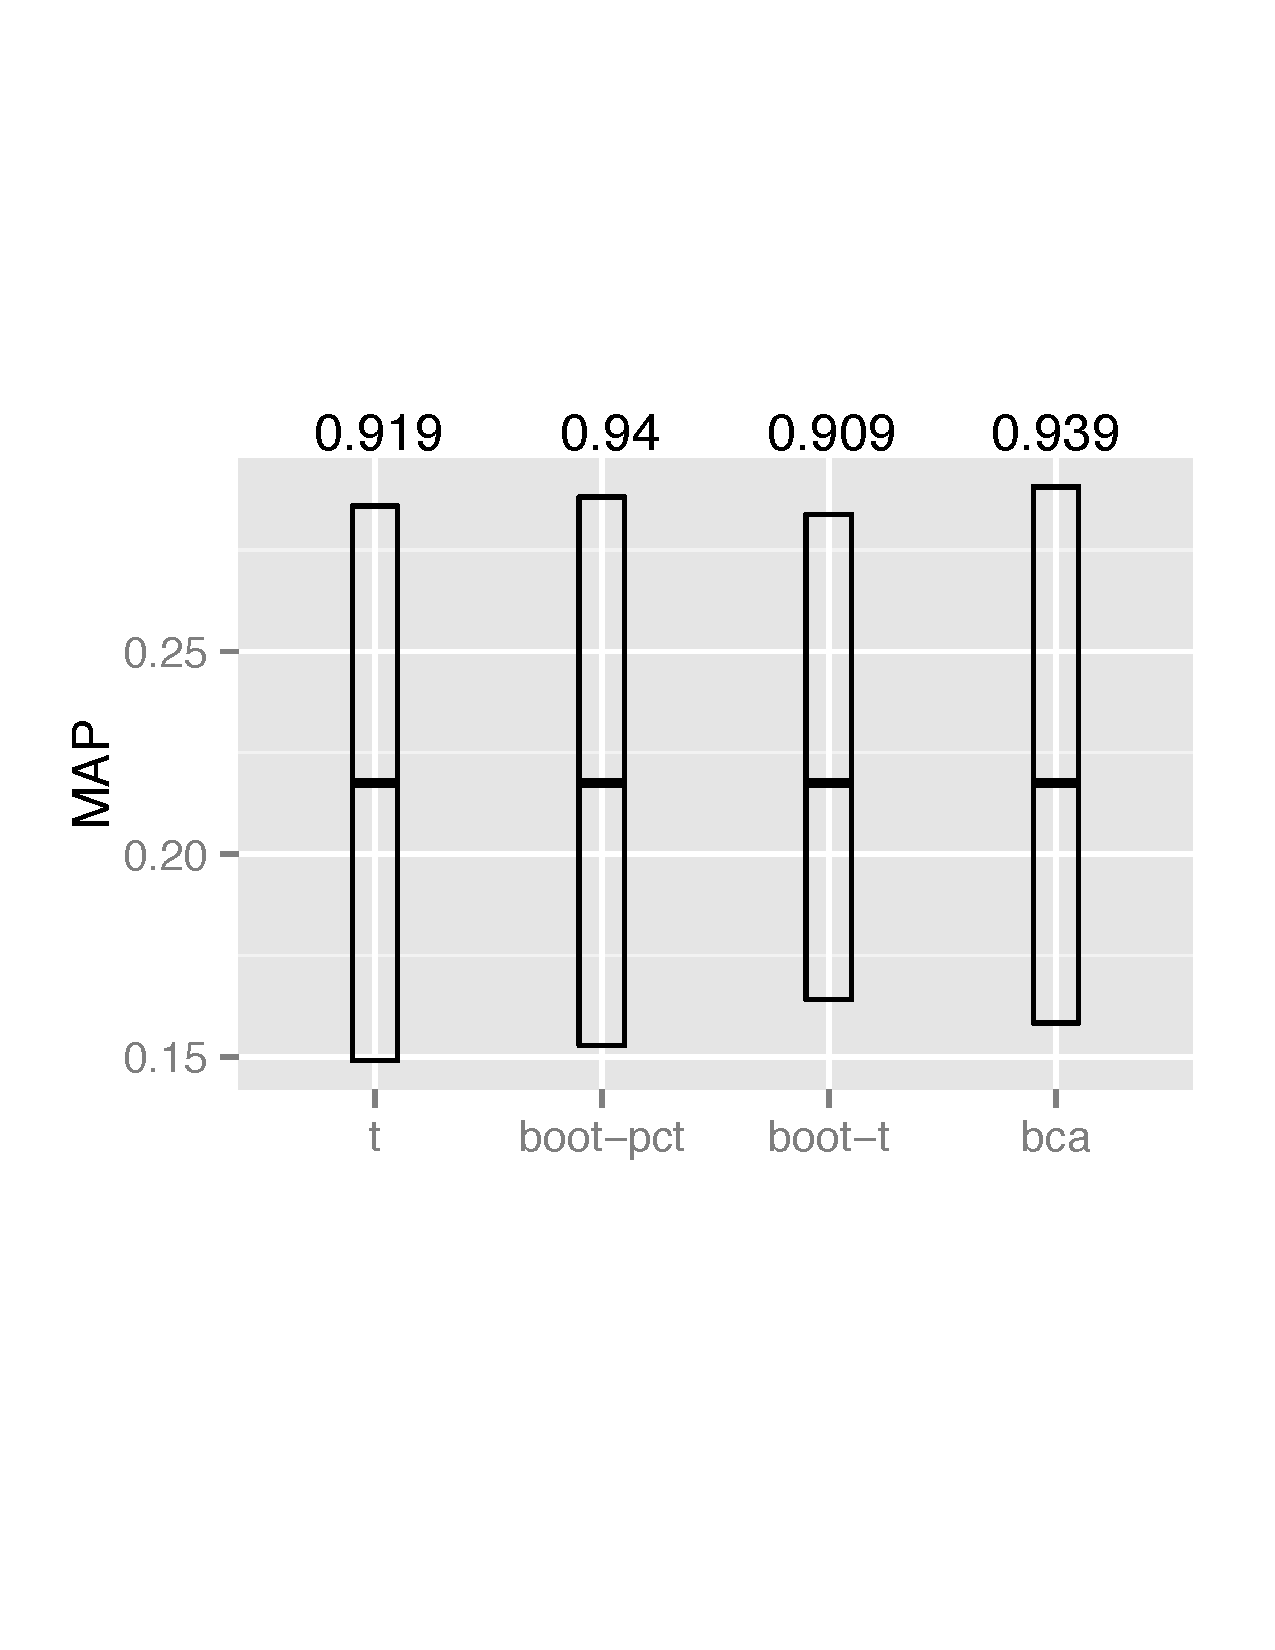
\includegraphics[width=\linewidth]{weaver1}
\caption{\label{run}Confidence intervals and empirical coverage probabilities for one example run and measure.}
\end{figure}

Figure~\ref{run} shows the confidence intervals for the mean average precision of the {\em weaver1} run.  The box range is the confidence interval, and the horizontal line is placed at the mean average precision, which is the same for all intervals, 0.2175.  The widths of the intervals are all roughly the same, with the bootstrap-$t$ interval slightly tighter.  The standard interval is symmetric about the mean, but the bootstrapped intervals can be asymmetric, extending farther in one direction or the other to capture the bootstrap distributions.

The empirical coverages of these intervals are shown above the boxes.  Again, the computed coverage values vary in practice due to sampling variation.  In this case the standard and bootstrap-$t$ intervals have equivalent coverage, but the bootstrap percentile and BCa intervals have coverage closer to the nominal confidence level. Following~\cite{Schall12} one can bootstrap a confidence interval on coverage, but we do not do that in this work.

\section{Experiments}

We would like to find out which method of computing confidence intervals gives the best empirical coverage, and hence best predictive value, for measures used in information retrieval research.  We computed standard, bootstrap percentile, bootstrap $t$, and BCa intervals at the 95\% level for mean average precision (MAP), R-precision, mean reciprocal rank, and precision at rank (10, 30, 1000) cutoffs.  We computed intervals for all official submitted runs for the TREC collections listed in Table~\ref{tab1}.  These collections were selected because they have common measures across a range of tasks, topic set sizes, and run set sizes.  Additionally, we computed confidence intervals for nDCG, nERR, and Q measure in the NTCIR-7 IR4QA collection; and for $\alpha$-nDCG, D-nDCG, D$\sharp$-nDCG, and nERR-IA in the NTCIR-10 INTENT collection.

\begin{table}
\begin{tabular}{l|lll}
Collection & topics & runs \\ \hline
TREC 8 adhoc & 50 & 129 \\
TREC 2004 robust & 100 & 83 \\
TREC 2005 robust & 50 & 74 \\
TREC 2006 terabyte (adhoc task) & 150 & 61 \\
TREC 2008 blog (topic rel) & 150 & 232 \\
TREC 2012 web & 50 & 48 \\
NTCIR-7 IR4QA & 97 & 40 \\
NTCIR-10 INTENT & 100 & 24 \\
\end{tabular}
\caption{\label{tab1}Details of test collections used in this paper.}
\end{table}

For each interval, we computed its empirical coverage probability using the bootstrap algorithm above.  A suitable confidence interval will have high coverage close to the nominal confidence level of the interval.  The scores and confidence interval data, along with Python code to compute all four intervals, is available from \url{https://github.com/isoboroff/confint}.

\section{Results}

The plots in figures~\ref{results-1} and~\ref{results-2} show the spread of empirical coverage rates for the different confidence intervals that we computed over the measures we examine across eight test collections.  The coverage spread is shown with a boxplot of the empirical coverage of the confidence interval over all runs in that collection.  The box extends over the interquartile distance and any points shown are outliers.

\begin{figure}
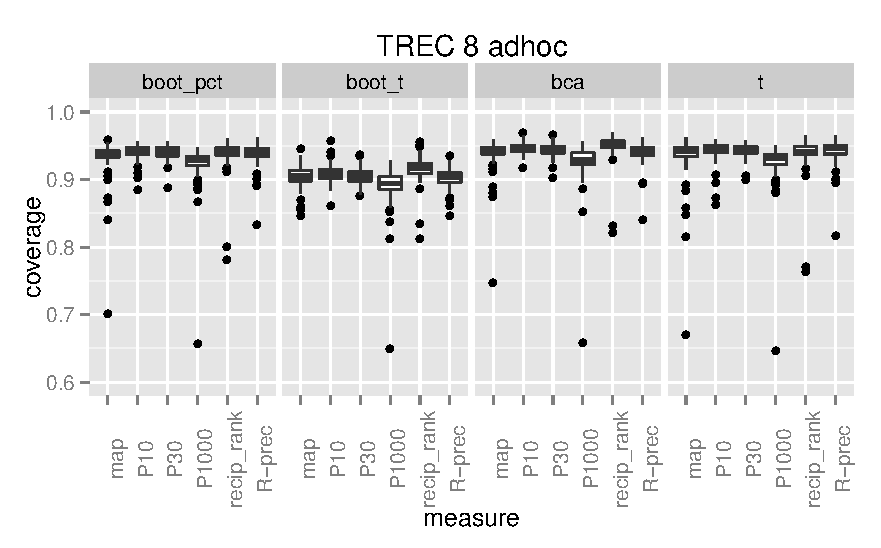
\includegraphics[width=\linewidth]{trec8-adhoc}
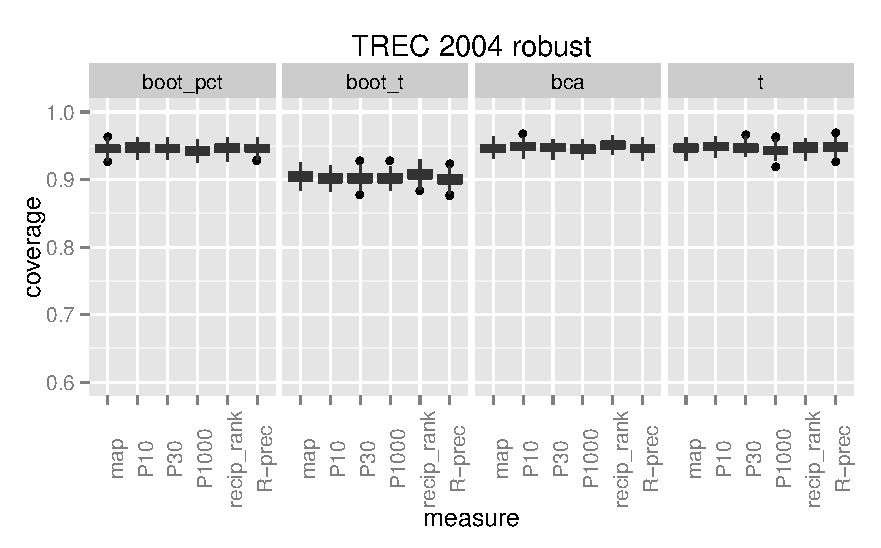
\includegraphics[width=\linewidth]{trec13-robust}
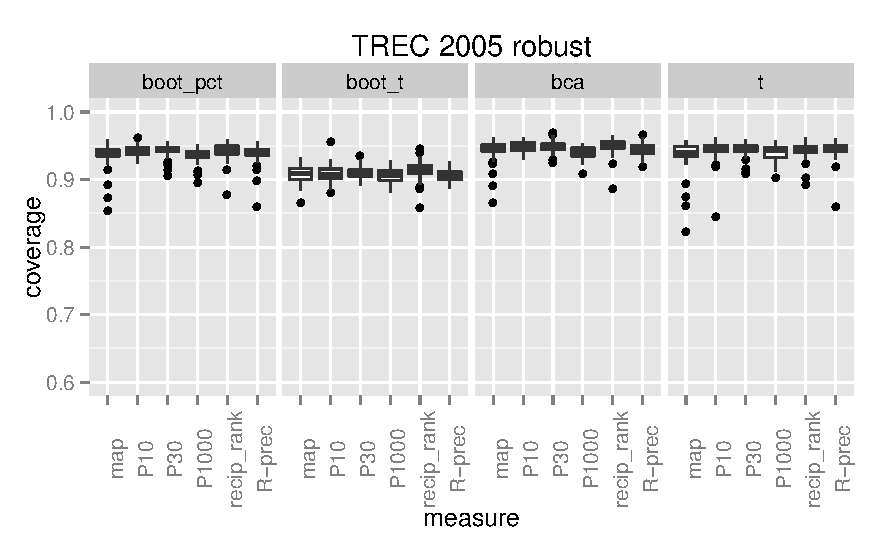
\includegraphics[width=\linewidth]{trec14-robust}
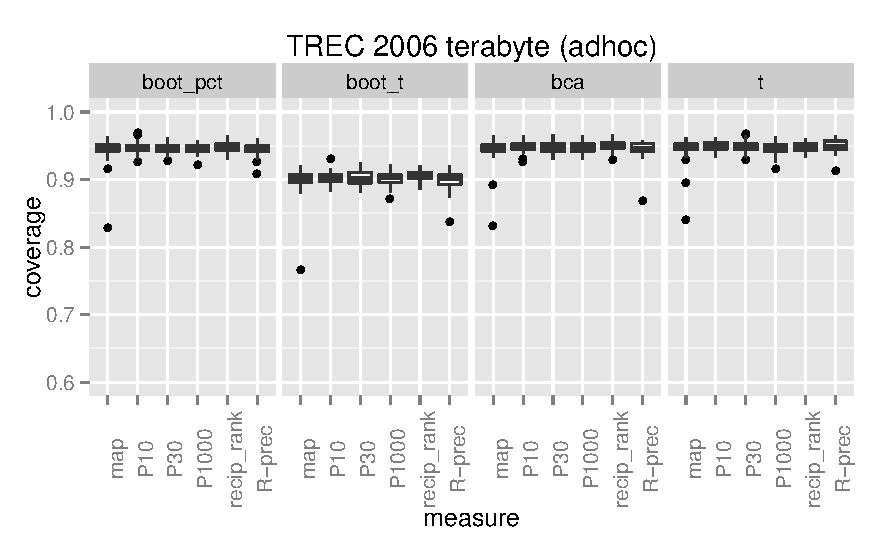
\includegraphics[width=\linewidth]{trec15-tb}
\caption{\label{results-1}Coverage results for different confidence intervals on IR measures in four TREC collections.}
\end{figure}

\begin{figure}
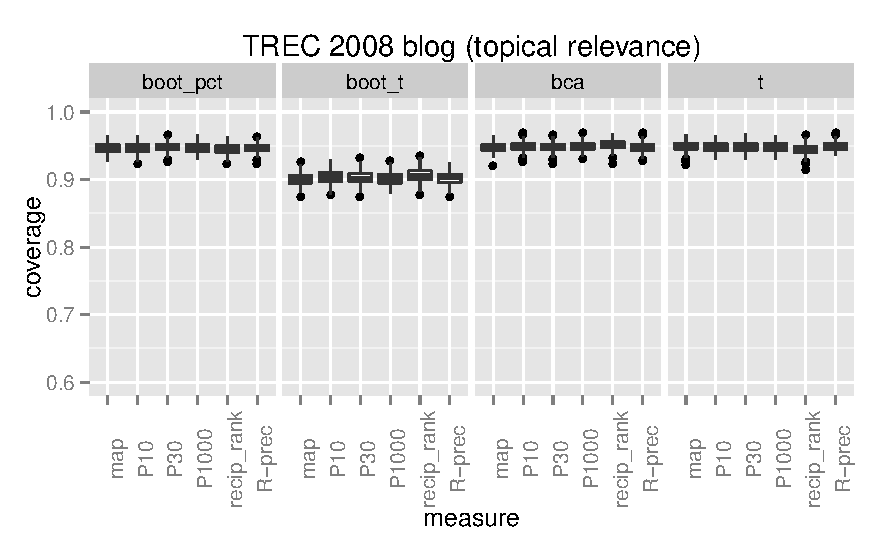
\includegraphics[width=\linewidth]{trec17-blog}
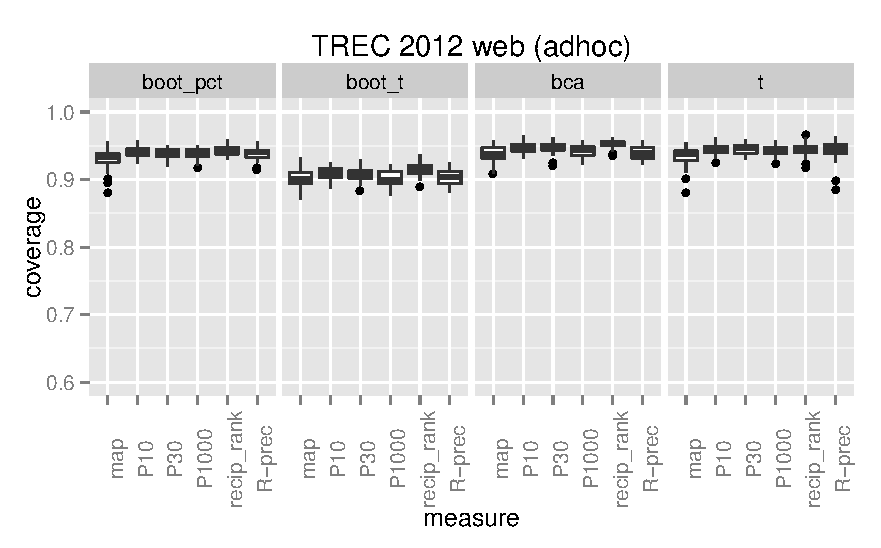
\includegraphics[width=\linewidth]{trec21-web}
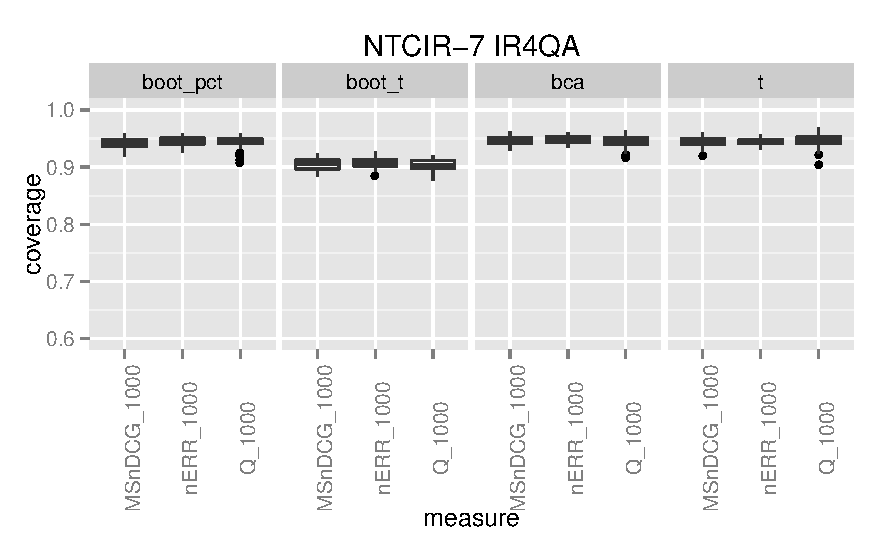
\includegraphics[width=\linewidth]{ntcir7-ir4qa}
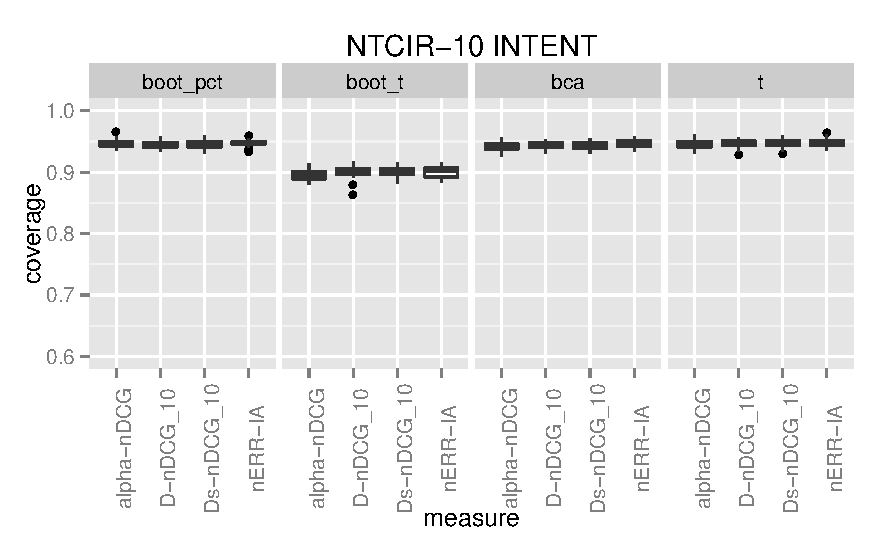
\includegraphics[width=\linewidth]{ntcir10-intent}
\caption{\label{results-2}(cont.) Coverage results for two more TREC collections and two NTCIR collections.}
\end{figure}

All of the interval methods have good empirical coverage close to the nominal confidence level.  The bootstrap-$t$ intervals have somewhat lower coverage, 0.9 on average across all collections and measures, compared to 0.94 -- 0.95 in the other methods.

In the TREC 8 adhoc, TREC 2005 robust, and TREC 2006 terabyte collections, there are some coverage outliers across all the measures.  These are situations where intervals give relatively poor coverage for some run/measure pairs.  From our inspection, this happens with runs that have scores of zero for most topics, and a few topics with nonzero scores.  For these runs, the bootstrap sampling methods are likely to draw topic subsets that contain only zeros, and the resulting confidence intervals are zero length.  The variance of this phenomenon across measures is due to how likely the measure is to quantize given a skewed sample of topic scores, and how far that resulting score would be from the true measured mean.

\section{Conclusion}

We explored four methods for computing confidence intervals on several information retrieval effectiveness measures in a wide range of test collections.  We found that all four methods give intervals with high empirical coverage of the true mean.  The bootstrap-$t$ method has lower coverage in our experiments and because of this we do not recommend its use for quantifying the uncertainty in these measures.

The bootstrap percentile method is trivially implemented in any programming language and does not require statistical library support.  The standard method is easily computed using textbook methods and common statistical software.  The BCa method is more complicated to implement, and since the bootstrap percentile and standard intervals seem to offer equivalent coverage, we do not see an advantage for these measures.

When seeking to compute confidence intervals for new measures and collections, we recommend the general approach taken in this paper, namely generating a range of parametric and nonparametric intervals and verifying their coverage empirically. Statisticians have formally investigated the coverage properties of these measures, but its simple enough to confirm explicitly what the data shows.

Just as increasing the number of topics in a collection can contribute to a successful significance test, using more topics results in tighter confidence intervals.  This indicates that larger topic sets are necessary to distinguish systems for some measures.  We plan to explore this in future work.

This paper discusses computing confidence intervals for single measures.  When comparing systems with a common test collection, confidence intervals may be directly compared during data analysis.  An alternative approach is to compute an interval on the mean difference between systems.  Like a paired $t$ test, intervals on the difference in means would be smaller than intervals on the measure itself.  Working with effect sizes rather than raw measure values is planned as future work.

\bibliography{confint}{}
\bibliographystyle{plain}



\end{document}
